\documentclass{beamer}
\usetheme[height=7mm]{Rochester}
\usepackage{listings}
\usepackage{url}

%\usefonttheme{serif}

\usepackage[T1]{fontenc}
\usepackage{inconsolata}

\usepackage[absolute,overlay]{textpos} 
\newenvironment{reference}[2]{% 
  \begin{textblock*}{\textwidth}(#1,#2) 
      \tiny\bgroup\color{red!50!black}}{\egroup\end{textblock*}} 

\def\UrlFont{\scriptsize\ttfamily}
\begin{document}

%%%%%%%%%%%%%%%%%%%%%%%%%%%%%%%%%%%%%%%%%%%%%%%%%%%%%%%%%%%%%%%%%%%%%%%%%%%%%%%%
%%%%%%%%%%%%%%%%%%%%%%%%%%%%%%%%%%%%%%%%%%%%%%%%%%%%%%%%%%%%%%%%%%%%%%%%%%%%%%%%
\title{Profile and reorder code execution in Geant4 to increase performance}
\subtitle{A Google Summer of Code Project}
\author{Stathis Kamperis}
\institute{
  Department of Physics\\
  Aristotle University of Thessaloniki\\
  Greece\\[1ex]
  \texttt{ekamperi@gmail.com}
}
\date{September, 2012}

%%%%%%%%%%%%%%%%%%%%%%%%%%%%%%%%%%%%%%%%%%%%%%%%%%%%%%%%%%%%%%%%%%%%%%%%%%%%%%%%
%%%%%%%%%%%%%%%%%%%%%%%%%%%%%%%%%%%%%%%%%%%%%%%%%%%%%%%%%%%%%%%%%%%%%%%%%%%%%%%%
\begin{frame}[plain]
  \titlepage
\end{frame}

%%%%%%%%%%%%%%%%%%%%%%%%%%%%%%%%%%%%%%%%%%%%%%%%%%%%%%%%%%%%%%%%%%%%%%%%%%%%%%%%
%%%%%%%%%%%%%%%%%%%%%%%%%%%%%%%%%%%%%%%%%%%%%%%%%%%%%%%%%%%%%%%%%%%%%%%%%%%%%%%%
\begin{frame}{Goals}
\begin{itemize}
\item {\bf Profile} Geant4 to identify potential targets of optimization (first half of GSoC period)
\item {\bf Reorder code execution} to improve serial performance (2nd half)
\end{itemize}
\textcolor{blue}{In reality} Goals were interchangeable
\end{frame}

%%%%%%%%%%%%%%%%%%%%%%%%%%%%%%%%%%%%%%%%%%%%%%%%%%%%%%%%%%%%%%%%%%%%%%%%%%%%%%%%
%%%%%%%%%%%%%%%%%%%%%%%%%%%%%%%%%%%%%%%%%%%%%%%%%%%%%%%%%%%%%%%%%%%%%%%%%%%%%%%%
\begin{frame}{Methods}
\begin{itemize}
\item {\bf Port of Geant4 to Solaris} 11/amd64 to access {\bf DTrace} profiling tool
\item {\bf Tool to compare 2 versions} of an application and generate an HTML report
\begin{itemize}
\item Tested on “FullCMS” and Simplified Calorimeter
\item Example (clickable): \url{http://island.quantumachine.net/~stathis/geant4/run-5550/smartstack.html}
\end{itemize}
\end{itemize}
\end{frame}

%%%%%%%%%%%%%%%%%%%%%%%%%%%%%%%%%%%%%%%%%%%%%%%%%%%%%%%%%%%%%%%%%%%%%%%%%%%%%%%%
%%%%%%%%%%%%%%%%%%%%%%%%%%%%%%%%%%%%%%%%%%%%%%%%%%%%%%%%%%%%%%%%%%%%%%%%%%%%%%%%
\begin{frame}{DTrace - Introduction 1/2}
\begin{itemize}
\item ``D'' stands for Dynamic- it dynamically instruments a running program,
by modifying its instructions while it is executing
\item {\bf Deep inspection}
\begin{itemize}
\item Arbitrary instructions
\item CPU registers
\item CPU hardware counters, etc
\end{itemize}
\item {\bf Sophisticated profiling} (e.g., speculative tracing)
\item {\bf Built-in aggregation} functions
\begin{itemize}
\item count, sum, avg, min, max, stddev, \{l,\}quantize
\end{itemize}

\item {\bf Negligible runtime overhead}
\end{itemize}
\end{frame}

%%%%%%%%%%%%%%%%%%%%%%%%%%%%%%%%%%%%%%%%%%%%%%%%%%%%%%%%%%%%%%%%%%%%%%%%%%%%%%%%
%%%%%%%%%%%%%%%%%%%%%%%%%%%%%%%%%%%%%%%%%%%%%%%%%%%%%%%%%%%%%%%%%%%%%%%%%%%%%%%%
\begin{frame}{DTrace - Introduction 2/2}
\begin{itemize}
\item {\bf Safe} to use in production environments
\begin{itemize}
\item Safety was one of the central architectural decisions upon DTrace was built
\item Explains why some common language constructs aren't supported (e.g., for-loops)
\end{itemize}

\item {\bf No source code modification} of the profiled application needed
\item Can operate on {\bf multithreaded} programs (has support for thread-local variables)
\item Runs on {\bf Mac OSX} out of the box; Linux port is on the way
\item Profiling done via a simple language called D (resembling C and awk)
\begin{itemize}
\item Scripts can be shared, reviewed, reused, made be run unattended
\end{itemize}
\end{itemize}
\end{frame}

%%%%%%%%%%%%%%%%%%%%%%%%%%%%%%%%%%%%%%%%%%%%%%%%%%%%%%%%%%%%%%%%%%%%%%%%%%%%%%%%
%%%%%%%%%%%%%%%%%%%%%%%%%%%%%%%%%%%%%%%%%%%%%%%%%%%%%%%%%%%%%%%%%%%%%%%%%%%%%%%%
\begin{frame}{Overview of ideas}

\textcolor{blue}{Some of the ideas explored}
\begin{itemize}
  \item {\bf Particle bunching (G4SmartTrackStack) }
  \item Caching of cross-sections calculations in hadronic processes (G4CrossSectionDataStore)  
  \item Reducing branch mispredictions in Value() (G4PhysicsVector)
  \item Hard-coded stepping manager (G4SteppingManager)  
  \item Caching values of ln(Energy) (G4Track)
\end{itemize}
\end{frame}

%%%%%%%%%%%%%%%%%%%%%%%%%%%%%%%%%%%%%%%%%%%%%%%%%%%%%%%%%%%%%%%%%%%%%%%%%%%%%%%%
%%%%%%%%%%%%%%%%%%%%%%%%%%%%%%%%%%%%%%%%%%%%%%%%%%%%%%%%%%%%%%%%%%%%%%%%%%%%%%%%
\begin{frame}{Particle "bunching" 1/2}
\textcolor{blue}{Definition}
Process \textit{same} particle types before switching to another particle type. E.g.,

\begin{equation*}
\ldots, e^-, e^-, \ldots, e^-, \gamma, \gamma, \ldots, \gamma, \ldots
\end{equation*}

\textcolor{blue}{Why} Better \textit{cache utilisation} due to access to the
same physics list

\vspace{5 mm}

4-5\% {\bf persistent} reduction in total execution time in FullCMS experiment (less in SimplifiedCalorimeter)

\end{frame}

%%%%%%%%%%%%%%%%%%%%%%%%%%%%%%%%%%%%%%%%%%%%%%%%%%%%%%%%%%%%%%%%%%%%%%%%%%%%%%%%
%%%%%%%%%%%%%%%%%%%%%%%%%%%%%%%%%%%%%%%%%%%%%%%%%%%%%%%%%%%%%%%%%%%%%%%%%%%%%%%%
\begin{frame}{Particle "bunching" 2/2}
\begin{center}
  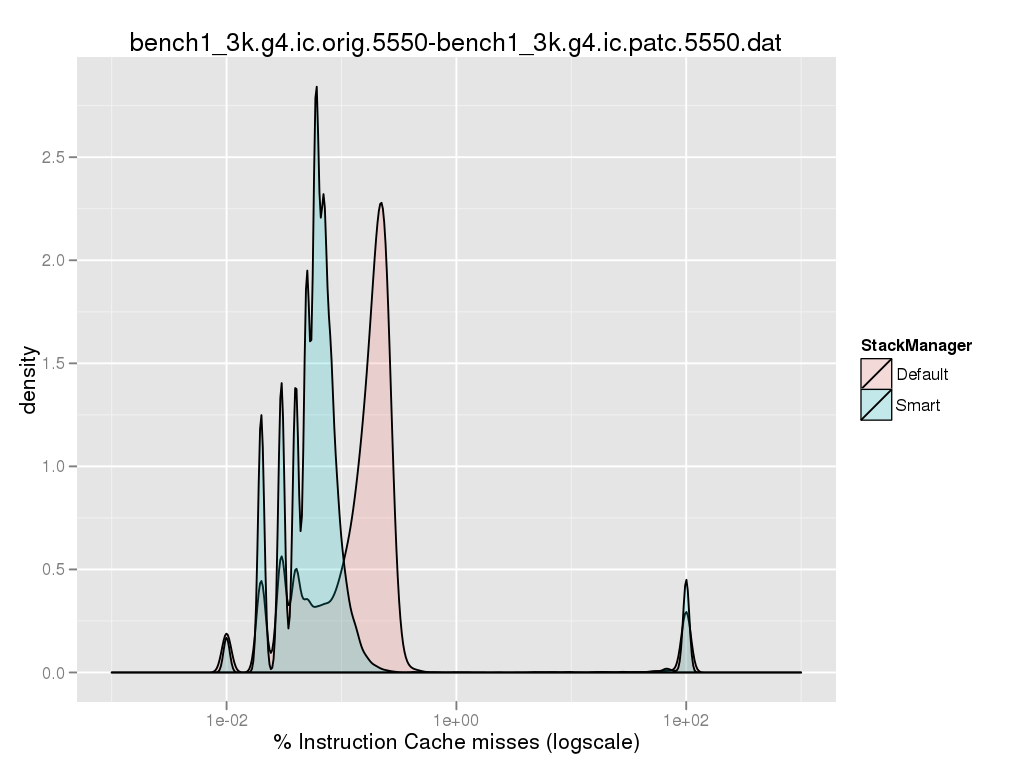
\includegraphics[width=1.0\textwidth]{histcmpicm.png}
\end{center}
\end{frame}

%%%%%%%%%%%%%%%%%%%%%%%%%%%%%%%%%%%%%%%%%%%%%%%%%%%%%%%%%%%%%%%%%%%%%%%%%%%%%%%%
%%%%%%%%%%%%%%%%%%%%%%%%%%%%%%%%%%%%%%%%%%%%%%%%%%%%%%%%%%%%%%%%%%%%%%%%%%%%%%%%
\begin{frame}{Speculative tracing - A real use case}

\textcolor{blue}{Problem} Some {\tt ProcessOneEvent()} need much more than
average time to complete

\begin{center}
  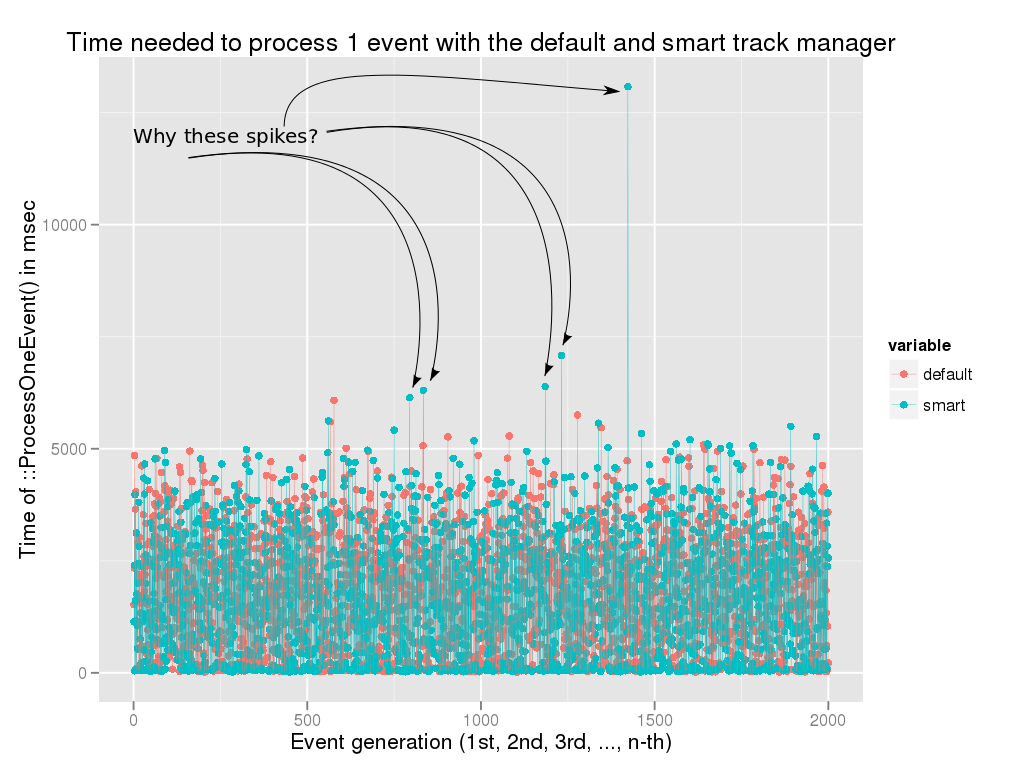
\includegraphics[width=0.8\textwidth]{evts1-arrows.png}
\end{center}
\end{frame}

%%%%%%%%%%%%%%%%%%%%%%%%%%%%%%%%%%%%%%%%%%%%%%%%%%%%%%%%%%%%%%%%%%%%%%%%%%%%%%%%
%%%%%%%%%%%%%%%%%%%%%%%%%%%%%%%%%%%%%%%%%%%%%%%%%%%%%%%%%%%%%%%%%%%%%%%%%%%%%%%%
\begin{frame}{Speculative tracing - A real use case}
\textcolor{blue}{Strategy} We are going to trace all {\tt ProcessOneEvent()} calls, but commit to our tracing
buffer \textit{only} those that behave bad.

\vspace{5mm}

In this context, "trace" refers to looking at stacks' sizes when {\tt ProcessOneEvent()}
stalls while processing the event.

\end{frame}

%%%%%%%%%%%%%%%%%%%%%%%%%%%%%%%%%%%%%%%%%%%%%%%%%%%%%%%%%%%%%%%%%%%%%%%%%%%%%%%%
%%%%%%%%%%%%%%%%%%%%%%%%%%%%%%%%%%%%%%%%%%%%%%%%%%%%%%%%%%%%%%%%%%%%%%%%%%%%%%%%
\begin{frame}{Speculative tracing - A real use case cont.}

\textcolor{blue}{Hint} The maximum desired size for all stacks was requested to be 400.

$e^-$ and $\gamma$ too often will not honour that limit.

\begin{center}
  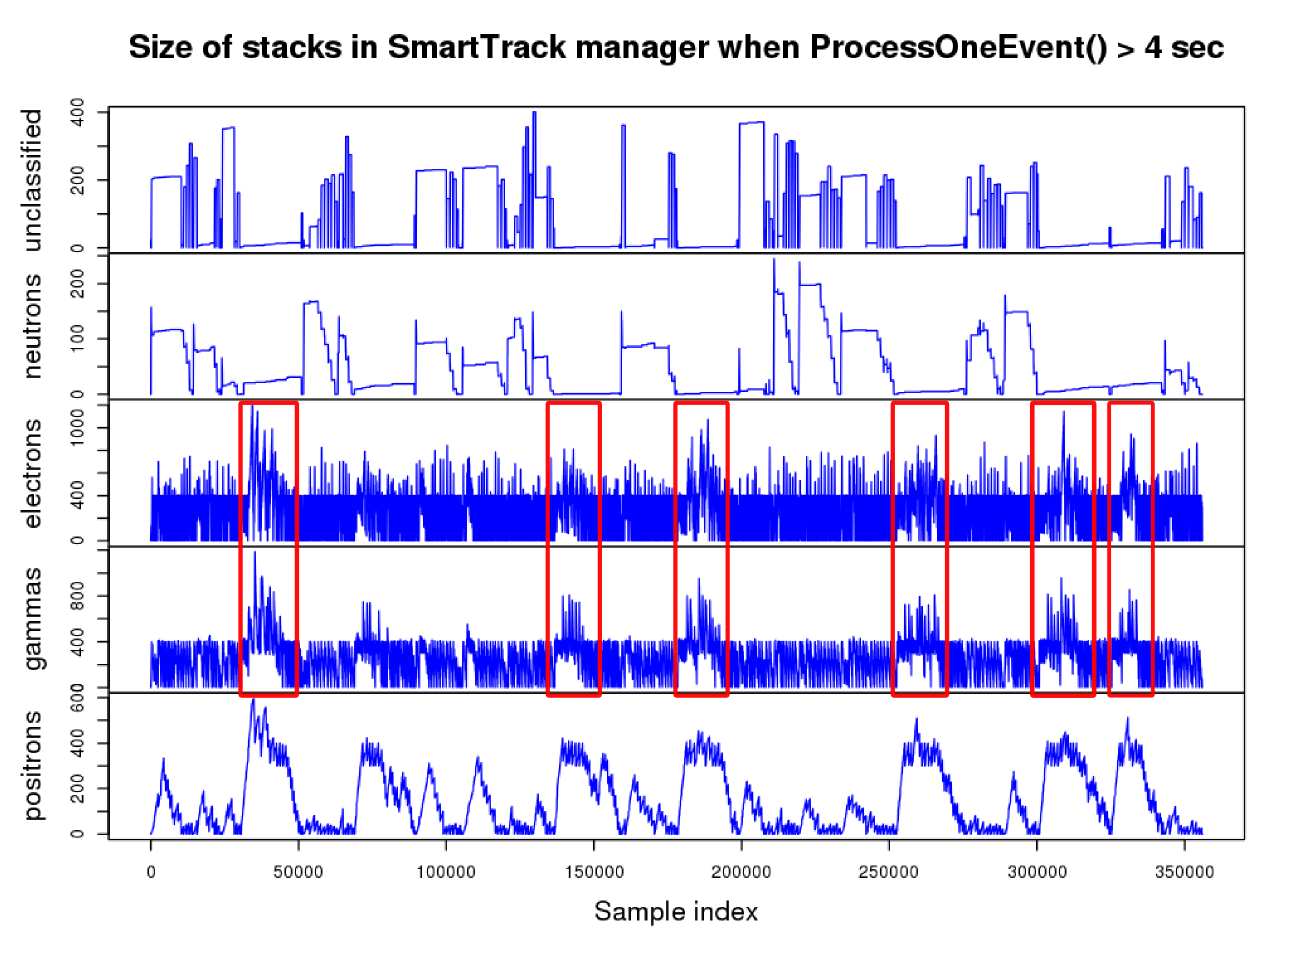
\includegraphics[width=0.8\textwidth]{pathol-all.png}
\end{center}
\end{frame}

%%%%%%%%%%%%%%%%%%%%%%%%%%%%%%%%%%%%%%%%%%%%%%%%%%%%%%%%%%%%%%%%%%%%%%%%%%%%%%%%
%%%%%%%%%%%%%%%%%%%%%%%%%%%%%%%%%%%%%%%%%%%%%%%%%%%%%%%%%%%%%%%%%%%%%%%%%%%%%%%%
\begin{frame}{Speculative tracing - A real use case cont. - Zoom 1/2}

\begin{center}
  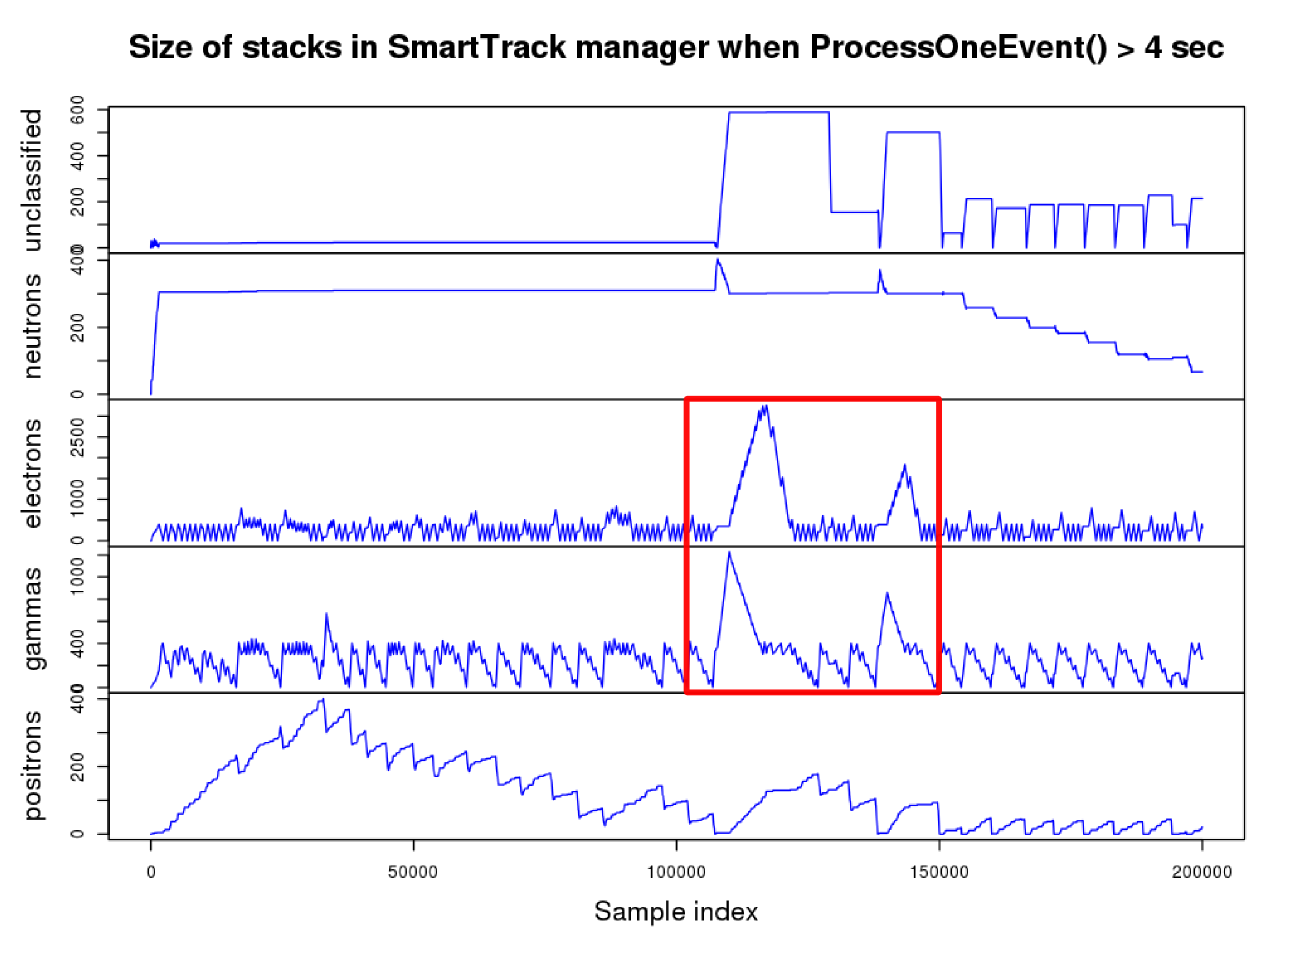
\includegraphics[width=0.8\textwidth]{pathol-zoom1.png}
\end{center}
\end{frame}


%%%%%%%%%%%%%%%%%%%%%%%%%%%%%%%%%%%%%%%%%%%%%%%%%%%%%%%%%%%%%%%%%%%%%%%%%%%%%%%%
%%%%%%%%%%%%%%%%%%%%%%%%%%%%%%%%%%%%%%%%%%%%%%%%%%%%%%%%%%%%%%%%%%%%%%%%%%%%%%%%
\begin{frame}{Caching cross-sections in hadronic processes}
\textcolor{blue}{Problem} A flamegraph showing CPU utilization identified
cross-section calculations in hadronic processes as a significant contributor

\vspace{5mm}

\textcolor{green}{Idea} Cache the values on some bin energy level

\vspace{5mm}

\textcolor{red}{Result} After many iterations, we have a version where the {\bf hits
ratio are very high} and there's {\bf probably a benefit of a few percent} (not yet quantified)

\vspace{5mm}

\textcolor{red}{TODO} Run enough simulations to extract the benefit. Study the
{\bf ramifications of bin'ing the energy} from the physics POV.

\end{frame}

%%%%%%%%%%%%%%%%%%%%%%%%%%%%%%%%%%%%%%%%%%%%%%%%%%%%%%%%%%%%%%%%%%%%%%%%%%%%%%%%
%%%%%%%%%%%%%%%%%%%%%%%%%%%%%%%%%%%%%%%%%%%%%%%%%%%%%%%%%%%%%%%%%%%%%%%%%%%%%%%%
\begin{frame}{Not all hadronic processes are cache-friendly 1/2}
\url {http://island.quantumachine.net/~stathis/geant4/hits}
\begin{center}
	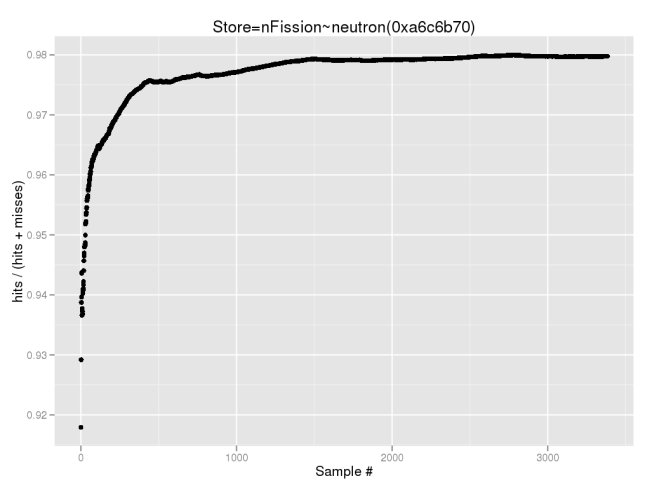
\includegraphics[width=1.0\textwidth]{002-2hits.png.medium.jpeg}
\end{center}
\end{frame}

%%%%%%%%%%%%%%%%%%%%%%%%%%%%%%%%%%%%%%%%%%%%%%%%%%%%%%%%%%%%%%%%%%%%%%%%%%%%%%%%
%%%%%%%%%%%%%%%%%%%%%%%%%%%%%%%%%%%%%%%%%%%%%%%%%%%%%%%%%%%%%%%%%%%%%%%%%%%%%%%%
\begin{frame}{Not all hadronic processes are cache-friendly 2/2}
\url {http://island.quantumachine.net/~stathis/geant4/hits}
\begin{center}
	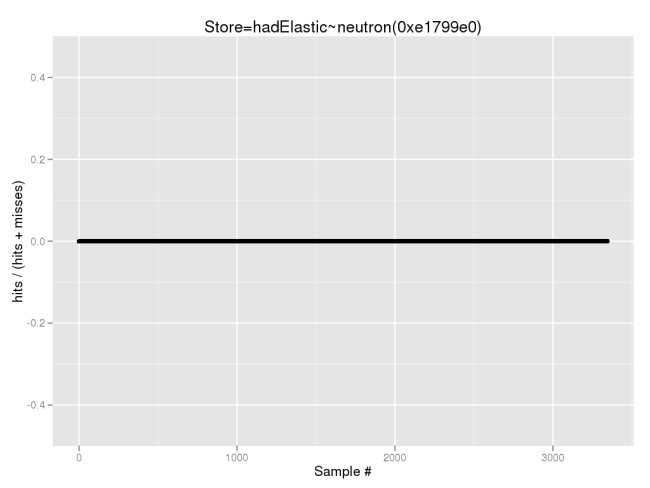
\includegraphics[width=1.0\textwidth]{003-3hits.png.medium.jpeg}
\end{center}
\end{frame}

%%%%%%%%%%%%%%%%%%%%%%%%%%%%%%%%%%%%%%%%%%%%%%%%%%%%%%%%%%%%%%%%%%%%%%%%%%%%%%%%
%%%%%%%%%%%%%%%%%%%%%%%%%%%%%%%%%%%%%%%%%%%%%%%%%%%%%%%%%%%%%%%%%%%%%%%%%%%%%%%%
\begin{frame}{Reducing branch mispredictions in G4PhysicsVector::Value()}

\textcolor{blue}{"Problem"} A flamegraph showing branch mispredictions identified
G4PhysicsVector::Value() as a significant offender

\vspace{5mm}

\textcolor{green}{Idea} Try to collapse some of the if-blocks, gaining branch
predictability, but executing more cpu instructions

\vspace{5mm}

\textcolor{red}{Result} The branch mispredictions reduced (expected), but the
average time spent in that function was actually larger

\end{frame}

%%%%%%%%%%%%%%%%%%%%%%%%%%%%%%%%%%%%%%%%%%%%%%%%%%%%%%%%%%%%%%%%%%%%%%%%%%%%%%%%
%%%%%%%%%%%%%%%%%%%%%%%%%%%%%%%%%%%%%%%%%%%%%%%%%%%%%%%%%%%%%%%%%%%%%%%%%%%%%%%%
\begin{frame}[fragile]{Reducing branch mispredictions in G4PhysicsVector::Value()}

\textcolor{blue}{Objective} Calculate the cache hits ratio in G4PhysicsVector::Value()

\lstset{basicstyle=\tiny\ttfamily}
\lstset{frame=single, columns=flexible}
\begin{lstlisting}
# dtrace -qn '
/* 0xc0 is the offset inside Value() where a fast cache hit takes place */
pid$target::_ZN15G4PhysicsVector5ValueEd:c0
{ 
    @branch = count();
}

pid$target::_ZN15G4PhysicsVector5ValueEd:entry
{
    @total = count();
}

tick-100ms
{
    printa(@branch);
    printa(@total);
}' -c '/home/stathis/geant4.9.5.p01/bin/full_cms ./bench1_5k.g4' -o val
\end{lstlisting}
\end{frame}

%%%%%%%%%%%%%%%%%%%%%%%%%%%%%%%%%%%%%%%%%%%%%%%%%%%%%%%%%%%%%%%%%%%%%%%%%%%%%%%%
%%%%%%%%%%%%%%%%%%%%%%%%%%%%%%%%%%%%%%%%%%%%%%%%%%%%%%%%%%%%%%%%%%%%%%%%%%%%%%%%
\begin{frame}{Reducing branch mispredictions in G4PhysicsVector::Value()}
\begin{center}
  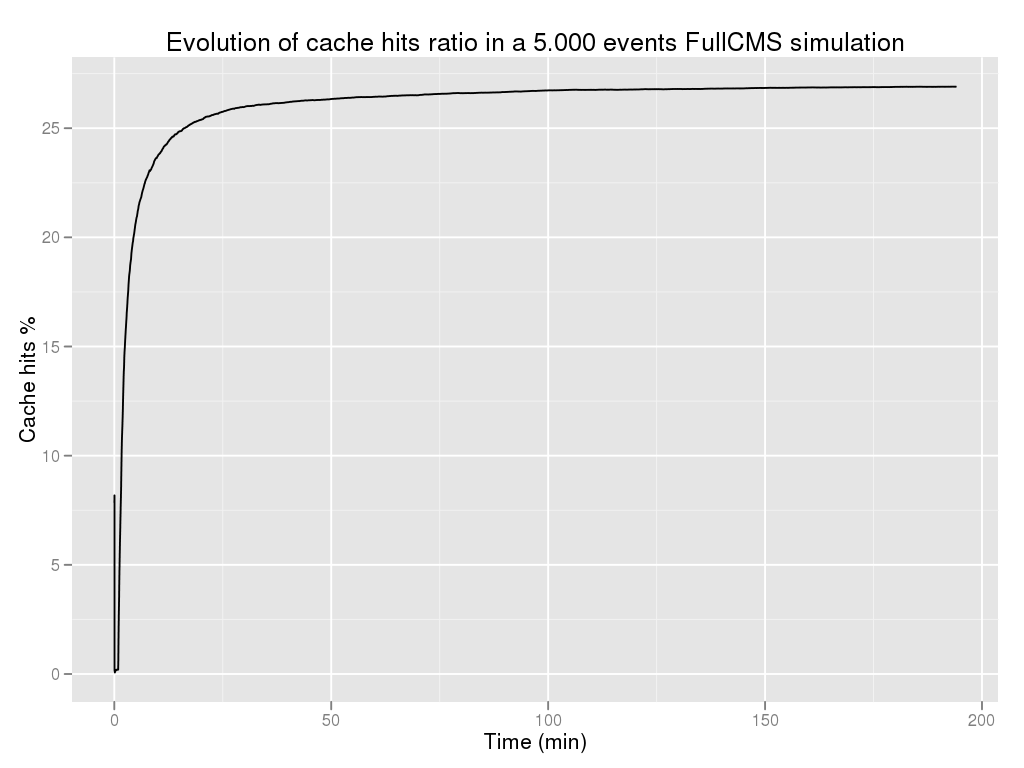
\includegraphics[width=1.0\textwidth]{G4PhysicsVector-Value.png}
\end{center}
\end{frame}

%%%%%%%%%%%%%%%%%%%%%%%%%%%%%%%%%%%%%%%%%%%%%%%%%%%%%%%%%%%%%%%%%%%%%%%%%%%%%%%%
%%%%%%%%%%%%%%%%%%%%%%%%%%%%%%%%%%%%%%%%%%%%%%%%%%%%%%%%%%%%%%%%%%%%%%%%%%%%%%%%
\begin{frame}{Reducing branch mispredictions in G4PhysicsVector::Value()}
\begin{itemize}
\item The benefit of caching outweighs (as reality dictates) the penalty of
branch mispredictions
\item The eventual ratio is higher than that I had initially in mind
\vspace{5mm}
\item {\bf Lesson learnt}: let the system reach its equilibrium before drawing any conclusions
\item {\bf Lesson learnt}: if you optimize 1 micro-benchmark, you may hurt another (or more)
\end{itemize}
\end{frame}

%%%%%%%%%%%%%%%%%%%%%%%%%%%%%%%%%%%%%%%%%%%%%%%%%%%%%%%%%%%%%%%%%%%%%%%%%%%%%%%%
%%%%%%%%%%%%%%%%%%%%%%%%%%%%%%%%%%%%%%%%%%%%%%%%%%%%%%%%%%%%%%%%%%%%%%%%%%%%%%%%
\begin{frame}{Reducing branch mispredictions in G4PhysicsVector::Value()}
Enter the "rabbit" hole\\
\begin{itemize}
\item \textcolor{blue}{Question} ::Value() has many distinct branches. How {\bf fast} are compared to each other ?
\vspace{5mm}
\item \textcolor{blue}{Question} ::Value() has many distinct branches. How {\bf many times} is each one executed ?
\end{itemize}
I will skip the DTrace script which is a bit long for a slide, but here are the graphs:
\end{frame}

%%%%%%%%%%%%%%%%%%%%%%%%%%%%%%%%%%%%%%%%%%%%%%%%%%%%%%%%%%%%%%%%%%%%%%%%%%%%%%%%
%%%%%%%%%%%%%%%%%%%%%%%%%%%%%%%%%%%%%%%%%%%%%%%%%%%%%%%%%%%%%%%%%%%%%%%%%%%%%%%%
\begin{frame}{How many times is each branch in ::Value() executed ?}
\begin{center}
  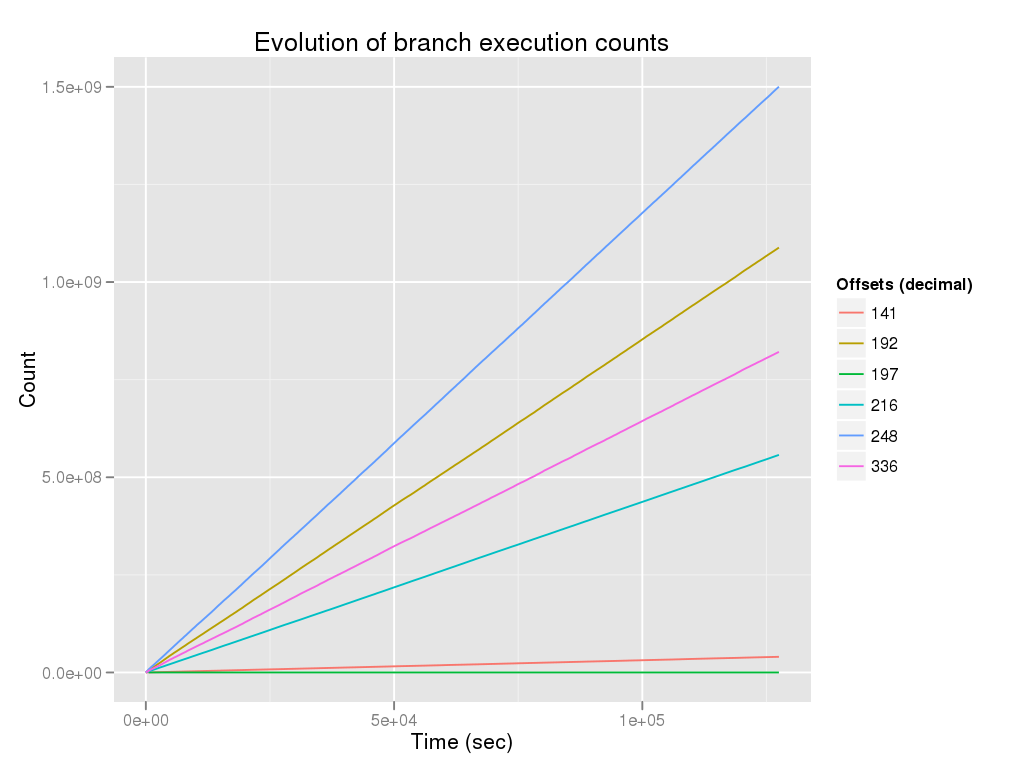
\includegraphics[width=1.0\textwidth]{branch-count.png}
\end{center}
\end{frame}

%%%%%%%%%%%%%%%%%%%%%%%%%%%%%%%%%%%%%%%%%%%%%%%%%%%%%%%%%%%%%%%%%%%%%%%%%%%%%%%%
%%%%%%%%%%%%%%%%%%%%%%%%%%%%%%%%%%%%%%%%%%%%%%%%%%%%%%%%%%%%%%%%%%%%%%%%%%%%%%%%
\begin{frame}{How fast are the branches in ::Value() compared to each other ?}
\begin{center}
  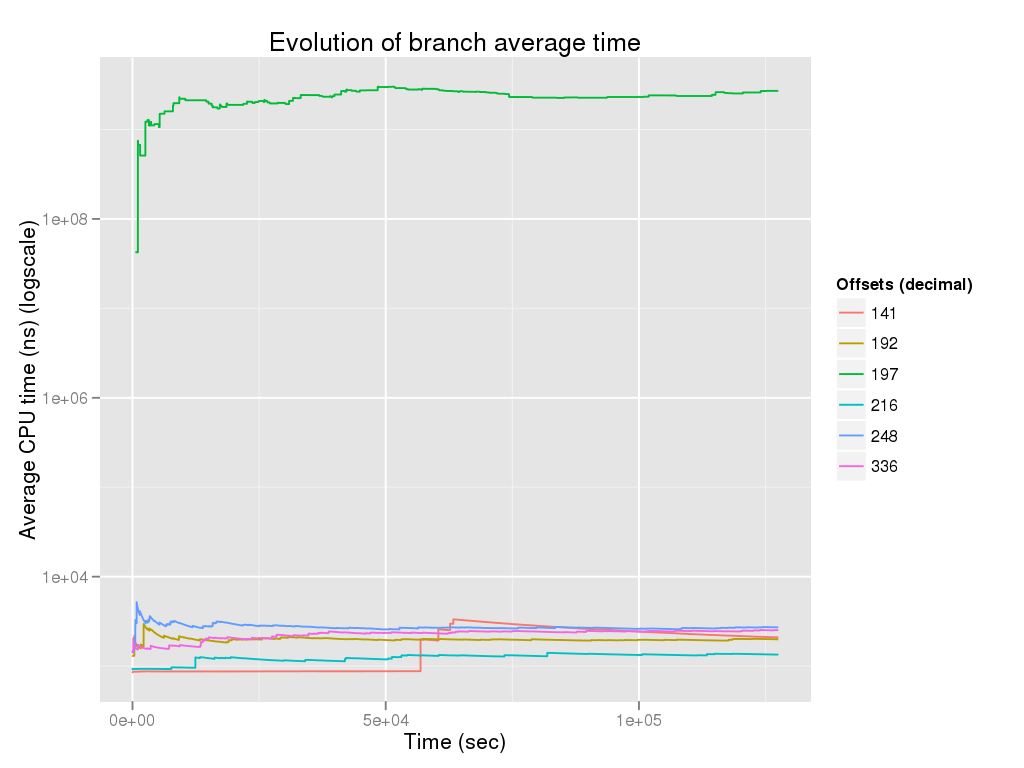
\includegraphics[width=1.0\textwidth]{branch-time.png}
\end{center}
\end{frame}

%%%%%%%%%%%%%%%%%%%%%%%%%%%%%%%%%%%%%%%%%%%%%%%%%%%%%%%%%%%%%%%%%%%%%%%%%%%%%%%%
%%%%%%%%%%%%%%%%%%%%%%%%%%%%%%%%%%%%%%%%%%%%%%%%%%%%%%%%%%%%%%%%%%%%%%%%%%%%%%%%
\begin{frame}{Hard-coded stepping manager (G4SteppingManager)}

\textcolor{blue}{Data} For some processes, \{AtRest, AlongStep, PostStep\}GPIL calls are placeholders.

\vspace{5mm}

\textcolor{green}{Idea} Replace them with direct hard-coded calls, instead of relying on compiled to do the dynamic dispatching

\vspace{5mm}

\textcolor{red}{Result} No detectable benefit. {\bf But}, it was done quickly, so it deserves further exploration

\end{frame}


%%%%%%%%%%%%%%%%%%%%%%%%%%%%%%%%%%%%%%%%%%%%%%%%%%%%%%%%%%%%%%%%%%%%%%%%%%%%%%%%
%%%%%%%%%%%%%%%%%%%%%%%%%%%%%%%%%%%%%%%%%%%%%%%%%%%%%%%%%%%%%%%%%%%%%%%%%%%%%%%%
\begin{frame}{Caching values of ln(Energy) (G4Track)}

\textcolor{blue}{Idea} Cache the logarithm of energy inside G4Track

\vspace{5mm}

\textcolor{green}{Exploration} A preliminary analysis with DTrace showed that the anticipated benefit would be less than 1\%

\vspace{5mm}

\textcolor{red}{Result} It hasn't been actively pursued until now
\end{frame}

%%%%%%%%%%%%%%%%%%%%%%%%%%%%%%%%%%%%%%%%%%%%%%%%%%%%%%%%%%%%%%%%%%%%%%%%%%%%%%%
%%%%%%%%%%%%%%%%%%%%%%%%%%%%%%%%%%%%%%%%%%%%%%%%%%%%%%%%%%%%%%%%%%%%%%%%%%%%%%%%
\begin{frame}{The end}
\vspace*{\fill}
\begin{center}
Thank you. Questions?
\end{center}
\vspace*{\fill}
\end{frame}

\end{document}
